\section{Results and Evaluation}

\subsection{Cross-Domain Validation Loss}

Table~\ref{tab:results} reports final validation loss and perplexity across
all seven domains at the end of each expansion stage.

\begin{table}[H]
\centering\small
\caption{Final validation loss / perplexity per domain and stage.  Bold
indicates the best result for each domain.  The target domain for each stage
is marked with $\star$.}
\label{tab:results}
\begin{tabular}{l|ccccc}
\toprule
\textbf{Domain} & \textbf{S2 (58M)} & \textbf{S3 (58M)} & \textbf{S4 (71M)}
& \textbf{S5 (71M)} & \textbf{S6 (100M)} \\
\midrule
TinyStories (s0)
  & \textbf{1.649} / 5.2  & 1.648 / 5.2  & 1.641 / 5.2
  & 1.697 / 5.5  & 1.667 / 5.3 \\
SimpleWiki (s1)
  & 7.516 / 1837 & 6.139 / 464  & \textbf{4.137}$^\star$ / \textbf{62.6}
  & 4.341 / 76.8 & 4.449 / 85.5 \\
FineWeb-Edu (s2)
  & 7.413 / 1657 & 6.070 / 433  & \textbf{5.210} / \textbf{183}
  & 5.244 / 189  & 5.312 / 203  \\
ROCStories (roc)
  & \textbf{2.711}$^\star$ / \textbf{15.0}
  & 3.259 / 26.0 & 3.577 / 35.8 & 3.609 / 36.9 & 3.630 / 37.7 \\
SimpleStories
  & \textbf{1.839} / \textbf{6.3}
  & 1.853 / 6.4  & 1.910 / 6.8  & 2.547 / 12.8 & 2.558 / 12.9 \\
Children (child)
  & 4.752 / 116  & \textbf{2.814}$^\star$ / \textbf{16.7}
  & 2.583 / 13.2 & 2.919 / 18.5 & 2.984 / 19.7 \\
WritingPrompts (wp)
  & 6.186 / 486  & 5.854 / 349  & 5.393 / 220
  & 3.797$^\star$ / 44.5
  & \textbf{3.743}$^\star$ / \textbf{42.1} \\
\bottomrule
\end{tabular}
\end{table}

\textbf{Key findings:}
\begin{itemize}[nosep]
  \item \textbf{TinyStories retention is excellent.}  Val loss stays between
        1.641 and 1.697 across all stages (baseline: 1.537).  The net
        degradation of ${\sim}0.13$ corresponds to a perplexity increase
        from 4.7 to 5.3---minimal given the model grew from 46M to 100M
        parameters and was trained on 5 new domains.
  \item \textbf{WritingPrompts drops from PPL 635 to 42.}  The staged approach
        successfully bridges the gap from children's stories to adult fiction.
  \item \textbf{SimpleWiki PPL drops from 2879 to 63.}  The introduction of
        encyclopedic text in Stage~4 dramatically improves factual language
        modeling.
  \item \textbf{ROCStories peaks at Stage~2.}  Since ROCStories is the
        target domain in Stage~2 and is gradually diluted in later stages,
        its val loss increases slightly (2.71$\to$3.63)---an expected
        trade-off of training on increasingly complex domains.
\end{itemize}

\subsection{Stage Summary}

\begin{table}[H]
\centering\small
\caption{Training summary per stage.}
\begin{tabular}{cccccl}
\toprule
\textbf{Stage} & \textbf{Steps} & \textbf{Tokens} & \textbf{Time} &
\textbf{Exit} & \textbf{Target Val} \\
\midrule
2 & 15{,}000 & 138M & 69 min & plateau & roc: 2.711 \\
3 & 15{,}000 & 138M & 69 min & plateau & child: 2.814 \\
4 & 15{,}000 & 123M & 77 min & plateau & s1: 4.137 \\
5 & 15{,}000 & 123M & 77 min & plateau & wp: 3.797 \\
6 & 15{,}000 &  92M & 79 min & plateau & wp: 3.743 \\
\bottomrule
\end{tabular}
\end{table}

Total training compute: $\sim$6.4 hours on a single NVIDIA RTX 4060 Ti (16~GB).

\subsection{Learning Curves}

\begin{figure}[H]
\centering
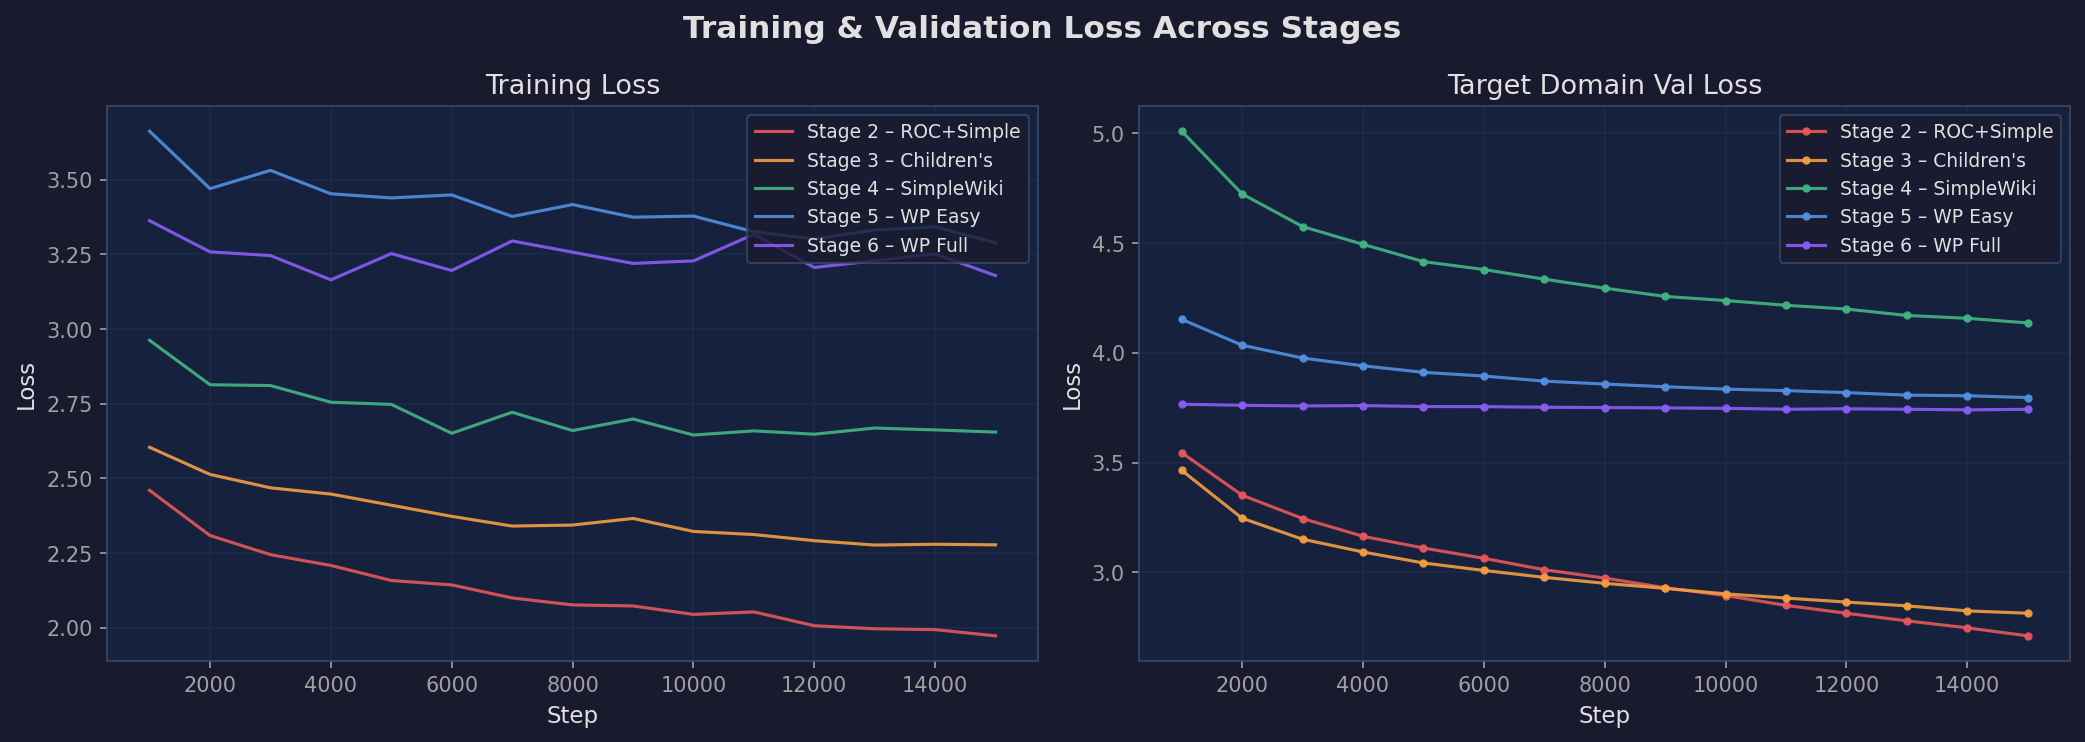
\includegraphics[width=\textwidth]{figures/01_train_val_loss.png}
\caption{Training loss (left) and target domain validation loss (right) across
all five expansion stages.  All stages converge smoothly; later stages have
higher absolute loss due to harder target domains.}
\label{fig:train_val}
\end{figure}

\begin{figure}[H]
\centering
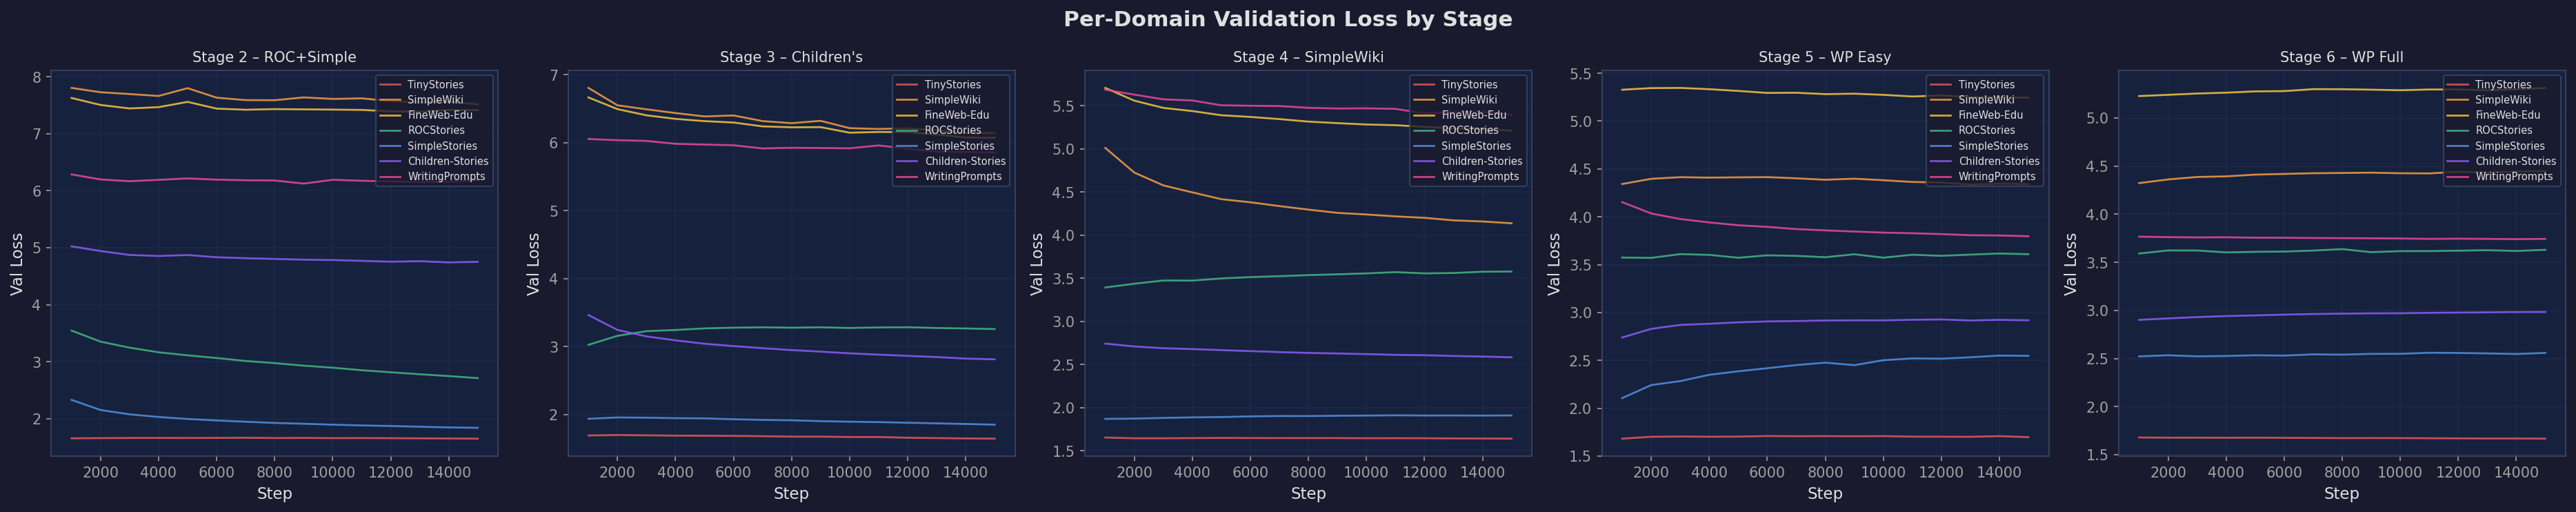
\includegraphics[width=\textwidth]{figures/02_domain_val_loss.png}
\caption{Per-domain validation loss breakdown for each stage.  Note how
TinyStories (red) remains consistently low across all stages, while the
target domain for each stage shows the steepest descent.}
\label{fig:domain_val}
\end{figure}

\begin{figure}[H]
\centering
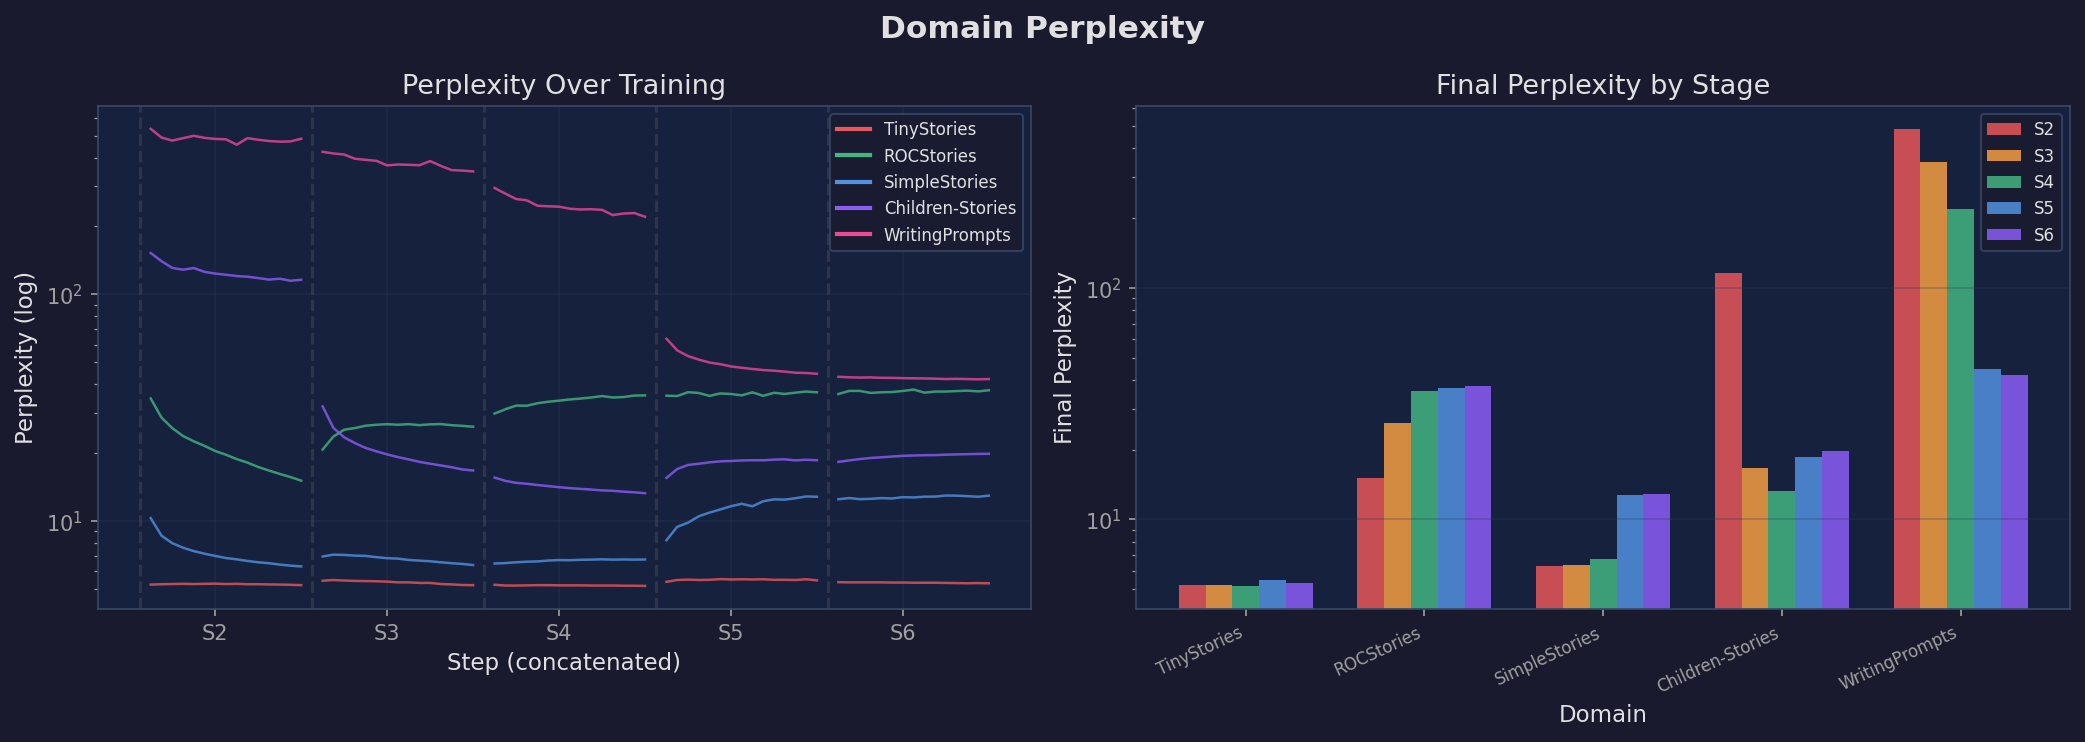
\includegraphics[width=\textwidth]{figures/03_domain_perplexity.png}
\caption{Left: log-scale perplexity over training (stages concatenated).
Right: final perplexity by domain and stage.  WritingPrompts and
Children-Stories show the most dramatic improvements.}
\label{fig:perplexity}
\end{figure}

\begin{figure}[H]
\centering
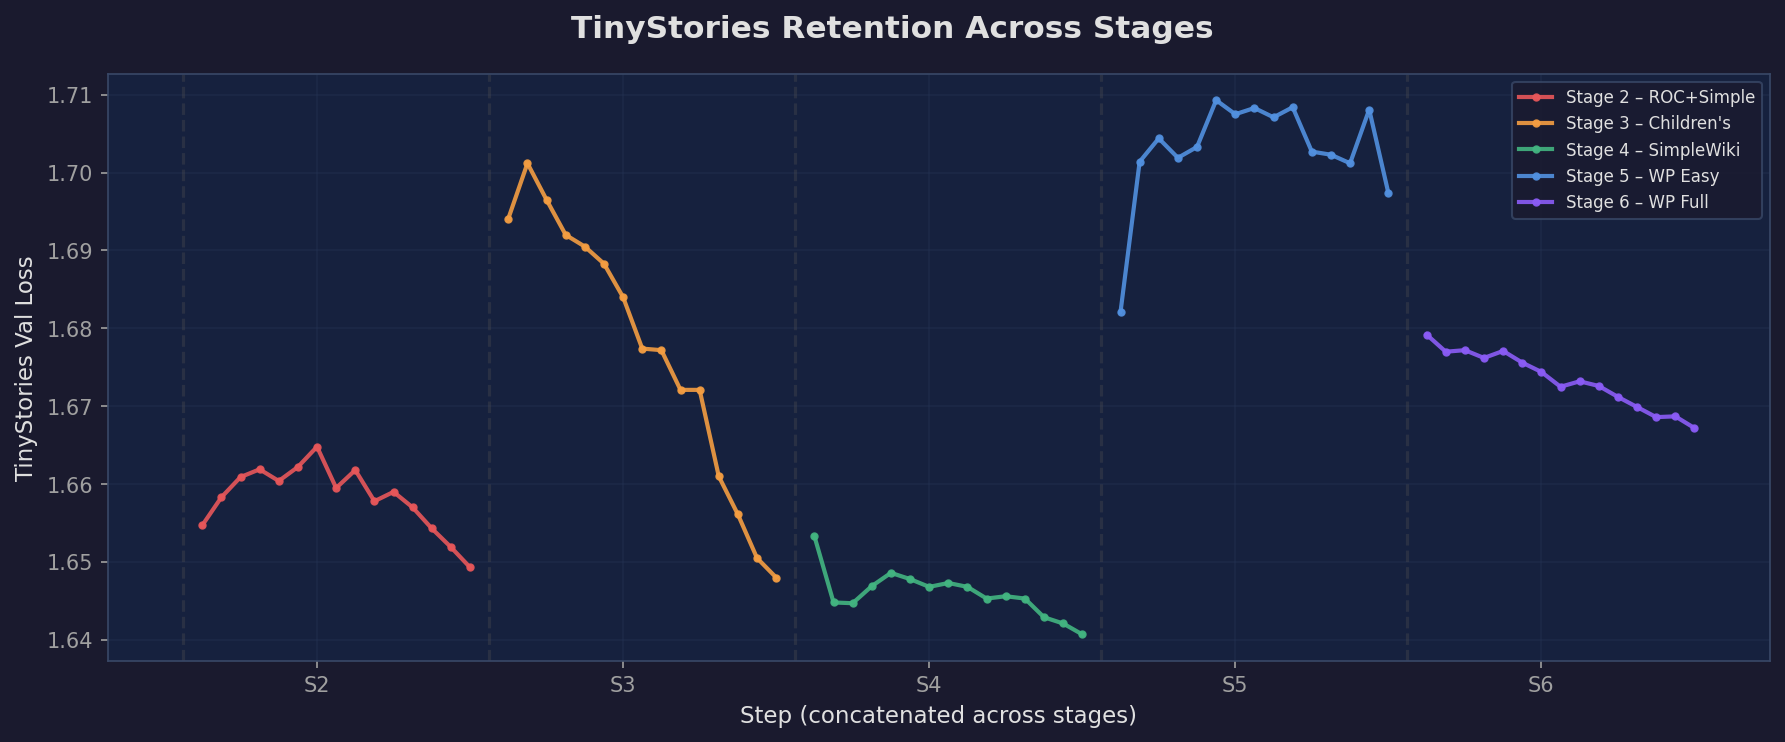
\includegraphics[width=\textwidth]{figures/09_tinystories_retention.png}
\caption{TinyStories validation loss across all stages, demonstrating stable
retention of the source domain.  The total range is only 1.64--1.71.}
\label{fig:retention}
\end{figure}

\begin{figure}[H]
\centering
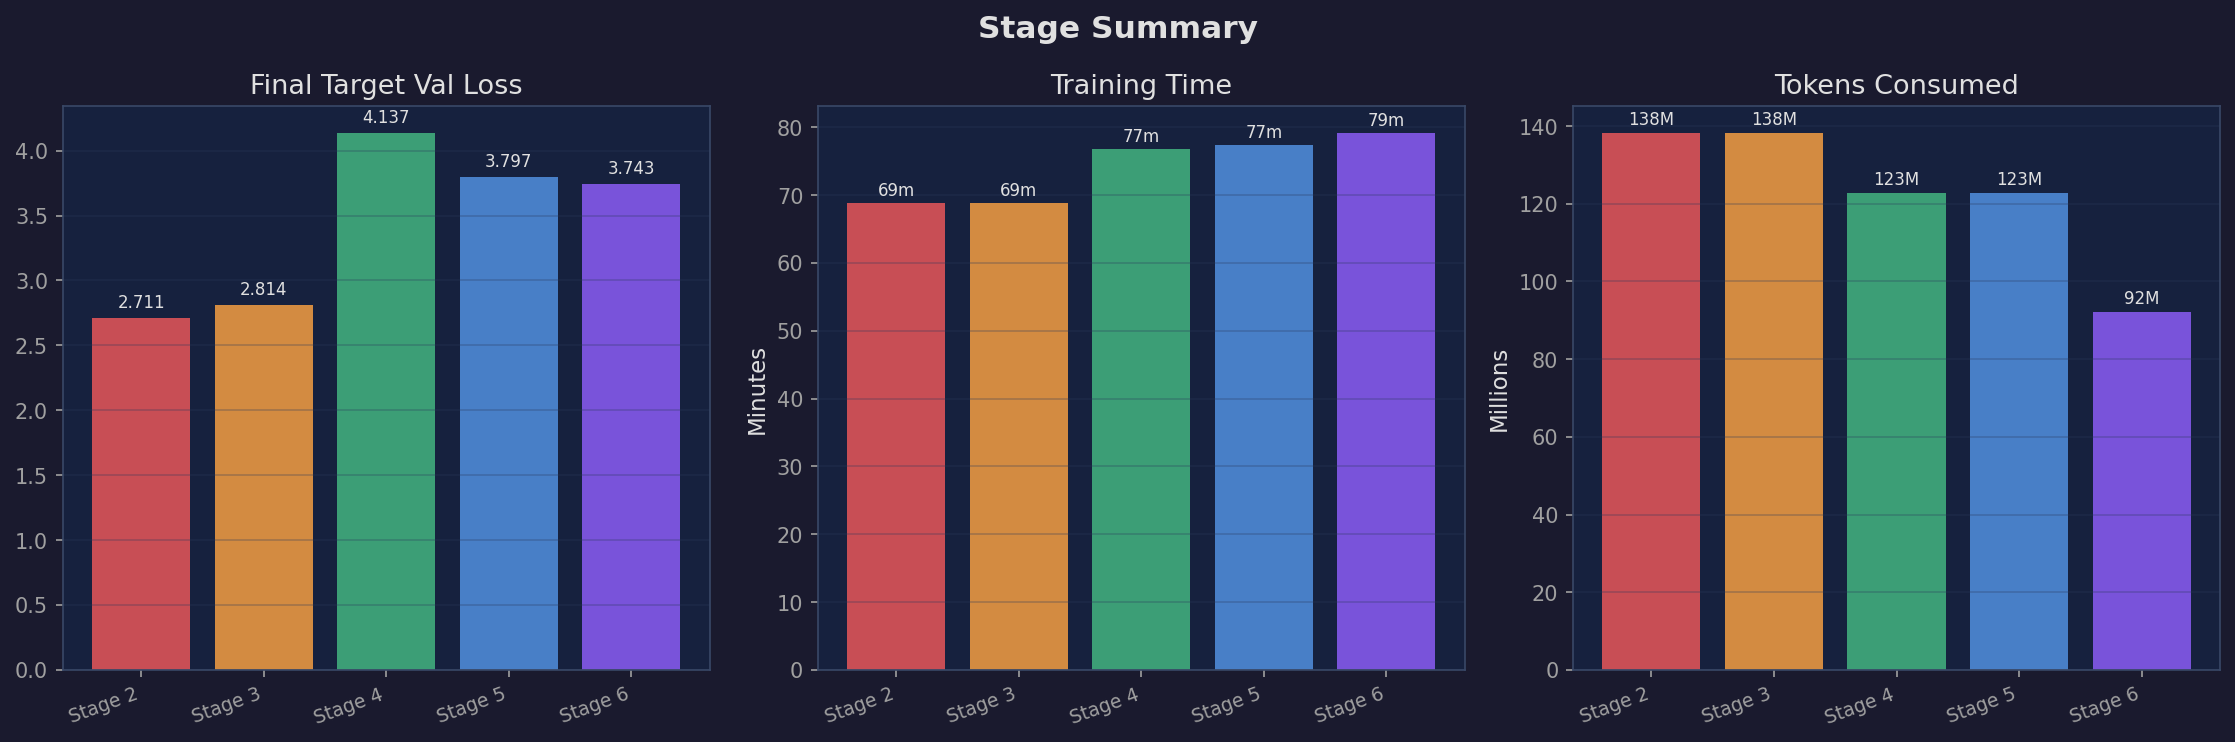
\includegraphics[width=\textwidth]{figures/08_stage_summary.png}
\caption{Stage-level summary: final target val loss, training time, and
tokens consumed.  Later stages process fewer tokens per step due to longer
sequences but take similar wall-clock time.}
\label{fig:summary}
\end{figure}

\begin{figure}[H]
\centering
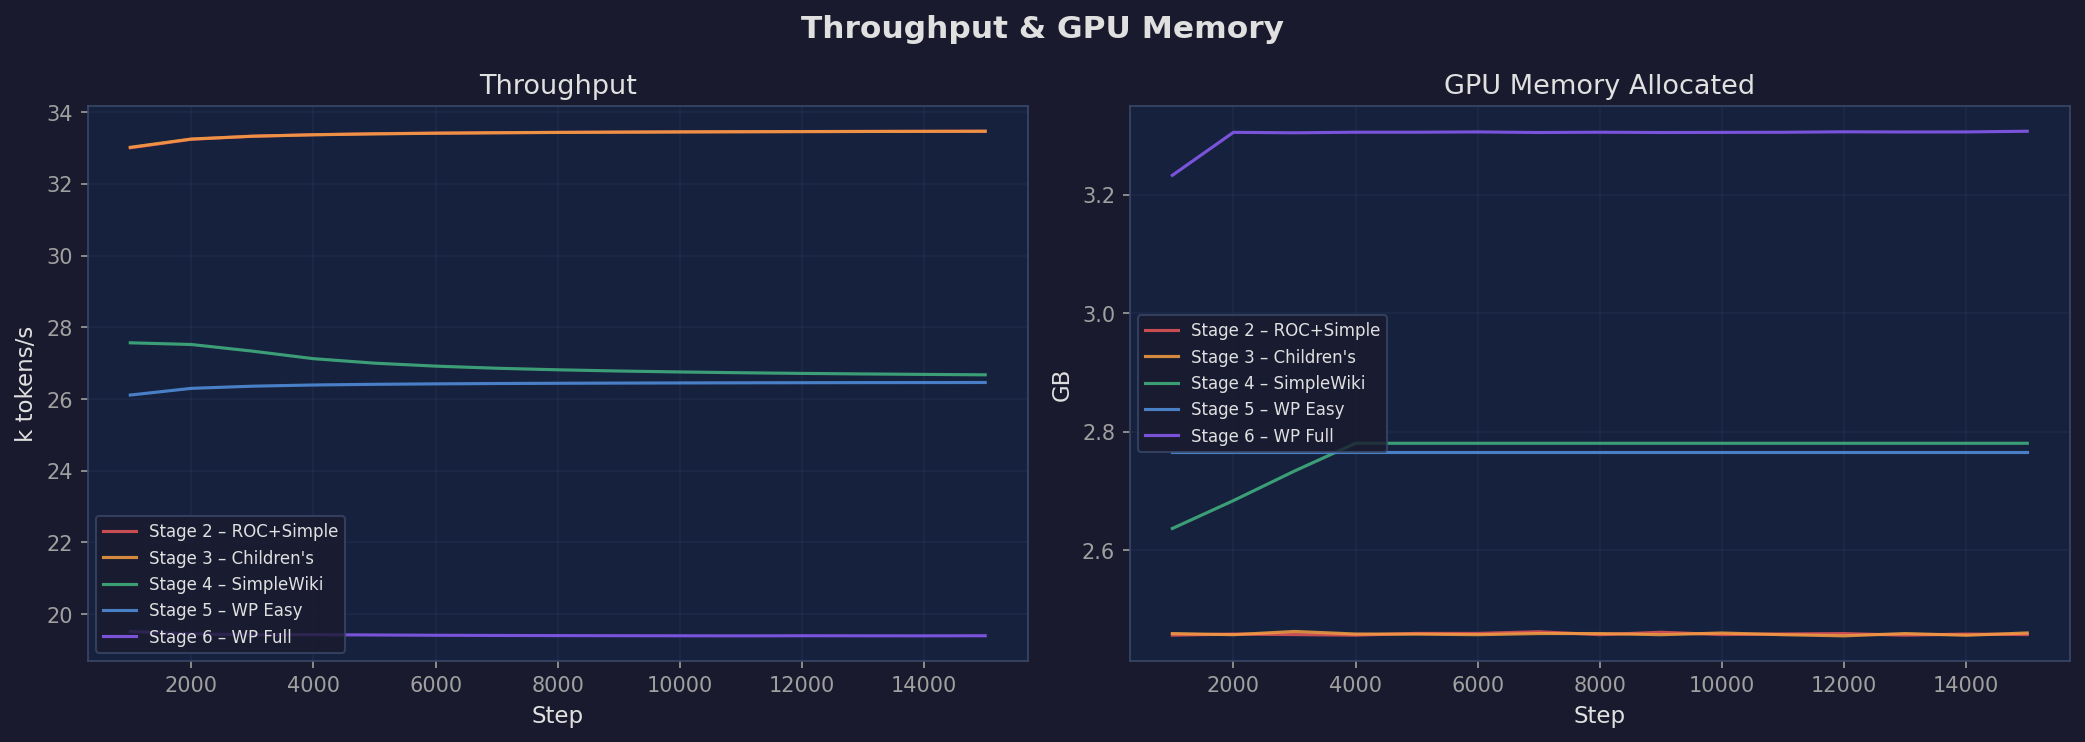
\includegraphics[width=\textwidth]{figures/06_throughput_memory.png}
\caption{Throughput (k tokens/s) and GPU memory allocation across stages.
Stages 4--5 (12 layers, seq 512) and Stage~6 (FFN 3584, seq 768) show
reduced throughput and increased memory usage, as expected.}
\label{fig:throughput}
\end{figure}
